\documentclass[11pt]{article}
\usepackage[margin=0.8in]{geometry}
\usepackage{amsmath,amssymb,booktabs,array,longtable}
\usepackage{graphicx}
\usepackage{float}
\usepackage{hyperref}
\usepackage{enumitem}
\setlist{nosep}

\begin{document}

\begin{center}
{\Large\textbf{Shiv Nadar University Chennai}}\\
\textbf{CS3807 -- Deep Learning Laboratory}\\
\textbf{Experiment 3}\\
{\large\textbf{Implementation of Convolutional Neural Networks (CNNs) for Image Classification}}
\end{center}

\renewcommand{\arraystretch}{1.25}

\begin{tabular}{|p{3.8cm}|p{8cm}|p{2cm}|}
\hline
Degree \& Branch & B.Tech Artificial Intelligence \& Data Science & Semester V\\ \hline
Subject Code \& Name & CS3807 -- Deep Learning Laboratory & AY: 2026--27\\ \hline
\end{tabular}

\section*{1. Objective}

To understand the working principle of Convolutional Neural Networks by implementing convolution, pooling, feature map visualization, and image classification using TensorFlow/Keras.

\section*{2. Learning Outcomes}

Students will be able to

\begin{enumerate}
\item Explain the convolution operation.
\item Compute output dimensions using stride and padding.
\item Visualize feature maps.
\item Implement max pooling and average pooling.
\item Calculate CNN parameters.
\item Build a CNN for image classification.
\item Evaluate CNN performance.
\end{enumerate}

\section*{3. Background Theory}

A Convolutional Neural Network consists of

\begin{itemize}
\item Convolution Layer
\item Activation Layer
\item Pooling Layer
\item Fully Connected Layer
\end{itemize}

The convolution operation is

\[
Y(i,j)=\sum_m\sum_n X(i+m,j+n)K(m,n)
\]

where

\begin{itemize}
\item $X$ : Input Image
\item $K$ : Kernel (Filter)
\item $Y$ : Feature Map
\end{itemize}

The output feature map size is

\[
\left\lfloor\frac{N-F+2P}{S}\right\rfloor+1
\]

where

\begin{tabular}{ll}
$N$ & Input Size\\
$F$ & Filter Size\\
$P$ & Padding\\
$S$ & Stride
\end{tabular}

\subsection*{3.1 Common Convolution Kernels}

A \textbf{kernel} (or \textbf{filter}) is a small matrix that slides over an input image to extract important visual features such as edges, textures, corners, and smooth regions. During convolution, the kernel is multiplied element-wise with the corresponding image pixels, and the results are summed to produce a single value in the output feature map. Different kernels highlight different image characteristics.

\subsubsection*{1. Identity Kernel}

The identity kernel preserves the original image without modifying its pixel values.

\[
\begin{bmatrix}
0 & 0 & 0\\
0 & 1 & 0\\
0 & 0 & 0
\end{bmatrix}
\]

\textbf{Purpose:}
\begin{itemize}
\item Preserves the original image.
\item Used for understanding the convolution operation.
\end{itemize}

\subsubsection*{2. Sobel-X Kernel (Vertical Edge Detection)}

The Sobel-X kernel detects \textbf{vertical edges} by measuring intensity changes along the horizontal direction.

\[
\begin{bmatrix}
-1 & 0 & 1\\
-2 & 0 & 2\\
-1 & 0 & 1
\end{bmatrix}
\]

\textbf{Applications:}
\begin{itemize}
\item Object detection
\item Lane detection
\item Face recognition
\end{itemize}

\subsubsection*{3. Sobel-Y Kernel (Horizontal Edge Detection)}

The Sobel-Y kernel detects \textbf{horizontal edges} by measuring intensity changes along the vertical direction.

\[
\begin{bmatrix}
-1 & -2 & -1\\
0 & 0 & 0\\
1 & 2 & 1
\end{bmatrix}
\]

\textbf{Applications:}
\begin{itemize}
\item Text detection
\item Boundary extraction
\item Medical image analysis
\end{itemize}

\subsubsection*{4. Laplacian Kernel}

The Laplacian kernel detects edges in all directions using the second-order derivative of image intensity.

\[
\begin{bmatrix}
0 & -1 & 0\\
-1 & 4 & -1\\
0 & -1 & 0
\end{bmatrix}
\]

\textbf{Applications:}
\begin{itemize}
\item Edge enhancement
\item Satellite image analysis
\item Medical imaging
\end{itemize}

\subsubsection*{5. Sharpening Kernel}

This kernel enhances fine details by emphasizing high-frequency components.

\[
\begin{bmatrix}
0 & -1 & 0\\
-1 & 5 & -1\\
0 & -1 & 0
\end{bmatrix}
\]

\textbf{Applications:}
\begin{itemize}
\item Image enhancement
\item Optical Character Recognition (OCR)
\item Face recognition
\end{itemize}

\subsubsection*{6. Box Blur Kernel}

The Box Blur kernel smooths an image by replacing each pixel with the average of its neighboring pixels.

\[
\frac{1}{9}
\begin{bmatrix}
1 & 1 & 1\\
1 & 1 & 1\\
1 & 1 & 1
\end{bmatrix}
\]

\textbf{Applications:}
\begin{itemize}
\item Noise removal
\item Image smoothing
\item Image preprocessing
\end{itemize}

\subsubsection*{7. Gaussian Blur Kernel}

Gaussian blur smooths the image while preserving the overall structure better than a simple average filter.

\[
\frac{1}{16}
\begin{bmatrix}
1 & 2 & 1\\
2 & 4 & 2\\
1 & 2 & 1
\end{bmatrix}
\]

\textbf{Applications:}
\begin{itemize}
\item Noise reduction
\item Computer vision preprocessing
\item Feature extraction
\end{itemize}

\subsubsection*{8. Emboss Kernel}

The Emboss kernel creates a three-dimensional appearance by emphasizing directional changes in intensity.

\[
\begin{bmatrix}
-2 & -1 & 0\\
-1 & 1 & 1\\
0 & 1 & 2
\end{bmatrix}
\]

\textbf{Applications:}
\begin{itemize}
\item Texture analysis
\item Artistic image effects
\end{itemize}

\subsubsection*{9. Outline Detection Kernel}

This kernel highlights object boundaries by emphasizing regions with rapid intensity changes.

\[
\begin{bmatrix}
-1 & -1 & -1\\
-1 & 8 & -1\\
-1 & -1 & -1
\end{bmatrix}
\]

\textbf{Applications:}
\begin{itemize}
\item Image segmentation
\item Boundary detection
\item Shape extraction
\end{itemize}

\subsubsection*{10. Motion Blur Kernel}

This kernel simulates motion blur along the diagonal direction.

\[
\frac{1}{5}
\begin{bmatrix}
1 & 0 & 0 & 0 & 0\\
0 & 1 & 0 & 0 & 0\\
0 & 0 & 1 & 0 & 0\\
0 & 0 & 0 & 1 & 0\\
0 & 0 & 0 & 0 & 1
\end{bmatrix}
\]

\textbf{Applications:}
\begin{itemize}
\item Motion simulation
\item Image restoration
\item Video processing
\end{itemize}

\subsubsection*{Summary of Common Kernels}

\begin{center}
\renewcommand{\arraystretch}{1.3}
\begin{tabular}{|p{3cm}|p{2cm}|p{4cm}|p{4cm}|}
\hline
\textbf{Kernel} & \textbf{Size} & \textbf{Purpose} & \textbf{Applications}\\
\hline
Identity & $3\times3$ & Preserve original image & Baseline comparison\\
\hline
Sobel-X & $3\times3$ & Detect vertical edges & Object detection\\
\hline
Sobel-Y & $3\times3$ & Detect horizontal edges & Boundary detection\\
\hline
Laplacian & $3\times3$ & Detect edges in all directions & Medical imaging\\
\hline
Sharpen & $3\times3$ & Enhance details & Image enhancement\\
\hline
Box Blur & $3\times3$ & Smooth image & Noise removal\\
\hline
Gaussian Blur & $3\times3$ & Reduce noise & Computer vision\\
\hline
Emboss & $3\times3$ & 3D effect & Artistic filtering\\
\hline
Outline & $3\times3$ & Boundary extraction & Segmentation\\
\hline
Motion Blur & $5\times5$ & Simulate motion & Video processing\\
\hline
\end{tabular}
\end{center}

\section*{4. Numerical Example 1: Convolution}

Consider the following input image.

\[
X=
\begin{bmatrix}
1&2&3\\
4&5&6\\
7&8&9
\end{bmatrix}
\]

Kernel

\[
K=
\begin{bmatrix}
1&0\\
0&1
\end{bmatrix}
\]

Output

First position

\[
1(1)+2(0)+4(0)+5(1)=6
\]

Second position

\[
2(1)+3(0)+5(0)+6(1)=8
\]

Third position

\[
4(1)+5(0)+7(0)+8(1)=12
\]

Fourth position

\[
5(1)+6(0)+8(0)+9(1)=14
\]

Feature Map

\[
\begin{bmatrix}
6&8\\
12&14
\end{bmatrix}
\]

\section*{5. Numerical Example 2: Max Pooling}

Feature map

\[
\begin{bmatrix}
1&5&2&3\\
7&8&1&0\\
4&6&9&5\\
2&3&1&8
\end{bmatrix}
\]

Using a $2\times2$ max pooling filter,

Window 1

\[
\begin{bmatrix}
1&5\\
7&8
\end{bmatrix}
\rightarrow 8
\]

Window 2

\[
\begin{bmatrix}
2&3\\
1&0
\end{bmatrix}
\rightarrow3
\]

Window 3

\[
\begin{bmatrix}
4&6\\
2&3
\end{bmatrix}
\rightarrow6
\]

Window 4

\[
\begin{bmatrix}
9&5\\
1&8
\end{bmatrix}
\rightarrow9
\]

Output

\[
\begin{bmatrix}
8&3\\
6&9
\end{bmatrix}
\]

\section*{6. Numerical Example 3: Parameter Calculation}

Suppose

Input Image

\[
32\times32\times3
\]

Convolution Layer

\begin{itemize}
\item Filters = 16
\item Kernel = $3\times3$
\end{itemize}

Parameters

\[
(3\times3\times3+1)\times16
\]

\[
=(27+1)\times16
\]

\[
=448
\]

Therefore,

Total trainable parameters = 448.

\section*{7. Dataset}

Dataset: CIFAR-10

\begin{itemize}
\item Training Images : 50,000
\item Testing Images : 10,000
\item Classes : 10
\item Image Size : $32\times32\times3$
\end{itemize}

\section*{8. Experimental Procedure}

\textbf{Task 1}

Load CIFAR-10.

\begin{itemize}
\item Display ten sample images.
\item Print dataset dimensions.
\item Plot class distribution.
\end{itemize}

\bigskip

\textbf{Task 2}

Implement a convolution layer.

Compare

\begin{itemize}
\item Kernel = $3\times3$
\item Kernel = $5\times5$
\item Kernel = $7\times7$
\end{itemize}

Record feature map sizes.

\bigskip

\textbf{Task 3}

Study hyperparameters.

Compare

\begin{itemize}
\item Stride = 1
\item Stride = 2
\item Padding = Same
\item Padding = Valid
\end{itemize}

Compute output dimensions.

\bigskip

\textbf{Task 4}

Visualize feature maps after the first convolution layer.

Display at least eight feature maps.

\bigskip

\textbf{Task 5}

Compare

\begin{itemize}
\item Max Pooling
\item Average Pooling
\end{itemize}

Compare output size and accuracy.

\bigskip

\textbf{Task 6}

Construct the following CNN.

\[
Input
\rightarrow
Conv
\rightarrow
ReLU
\rightarrow
MaxPool
\rightarrow
Conv
\rightarrow
ReLU
\rightarrow
MaxPool
\rightarrow
Flatten
\rightarrow
Dense
\rightarrow
Softmax
\]

Train for

\begin{itemize}
\item Optimizer : Adam
\item Epochs : 20
\item Batch Size : 32
\end{itemize}

\bigskip

\textbf{Task 7}

Evaluate

\begin{itemize}
\item Accuracy
\item Precision
\item Recall
\item F1-score
\item Confusion Matrix
\item Classification Report
\end{itemize}

\section*{9. Source Code}

The complete source code is attached separately in the GitHub repository and submitted along with this report.

\textbf{GitHub Repository:}

\url{https://github.com/Sadhana2006-art/Deep-Learning-Lab}

\section*{10. Plots with Inference}

\subsection*{10.1 Sample Images}

\begin{figure}[H]
\centering
\includegraphics[width=\textwidth]{Sample_images.eps}
\caption{Sample Images from the Dataset}
\end{figure}

\textbf{Interpretation:}

The picture has ten sample pictures from the CIFAR-10 dataset. These pictures show things like Frog, Truck, Deer, Automobile, Bird, Horse, Ship and Cat. Each picture is a picture, with $32\times32$ pixels.

\subsection*{10.2 Class Distribution}

\begin{figure}[H]
\centering
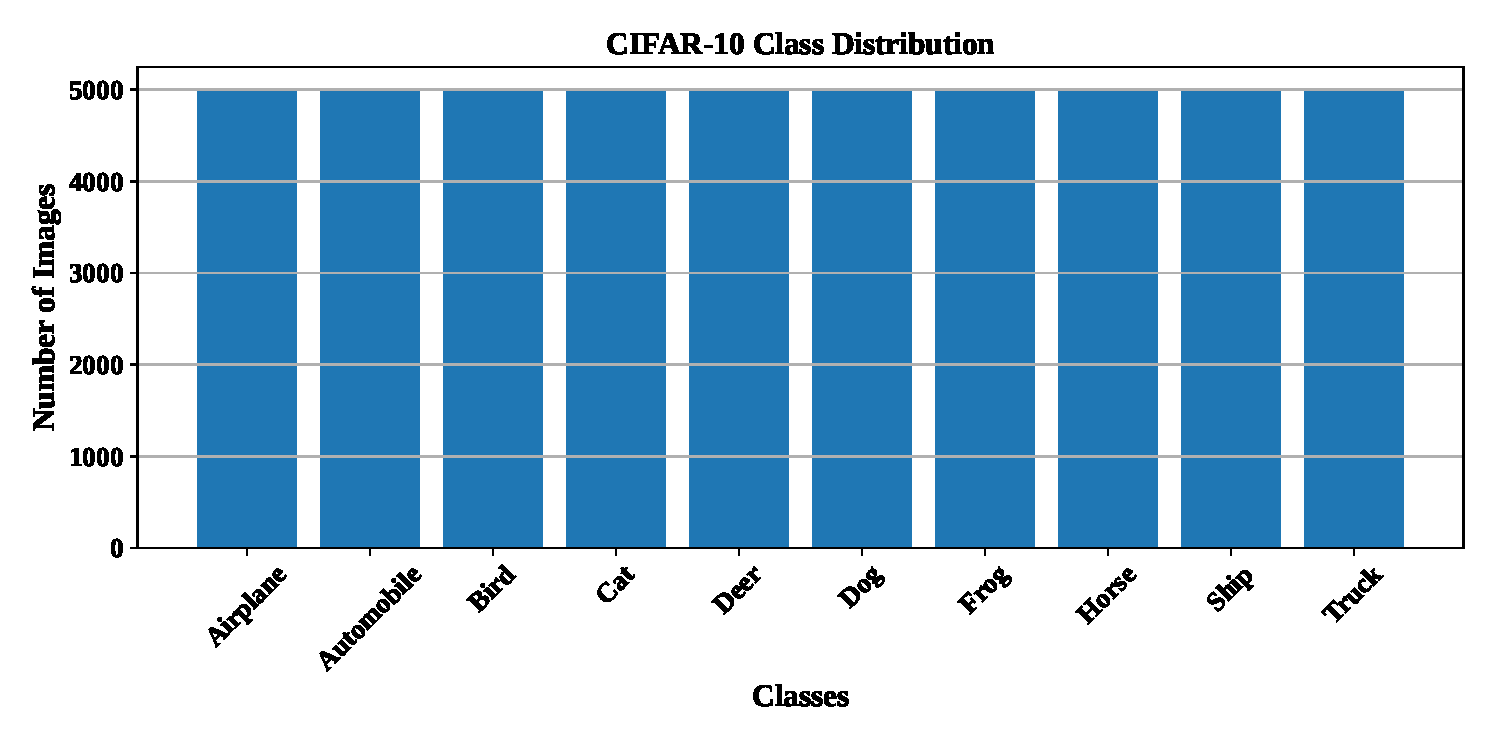
\includegraphics[width=\textwidth]{Class_distribution.eps}
\caption{Distribution of Classes in the Dataset}
\end{figure}

\textbf{Interpretation:}

The class distribution plot shows that each of the ten CIFAR-10 classes has 5,000 training images. The bars are equal in length. This means the training set is balanced. This balance prevents any class from being overrepresented in the training of the model. Training dataset is balanced.

\subsection*{10.3 Training Accuracy}

\begin{figure}[H]
\centering
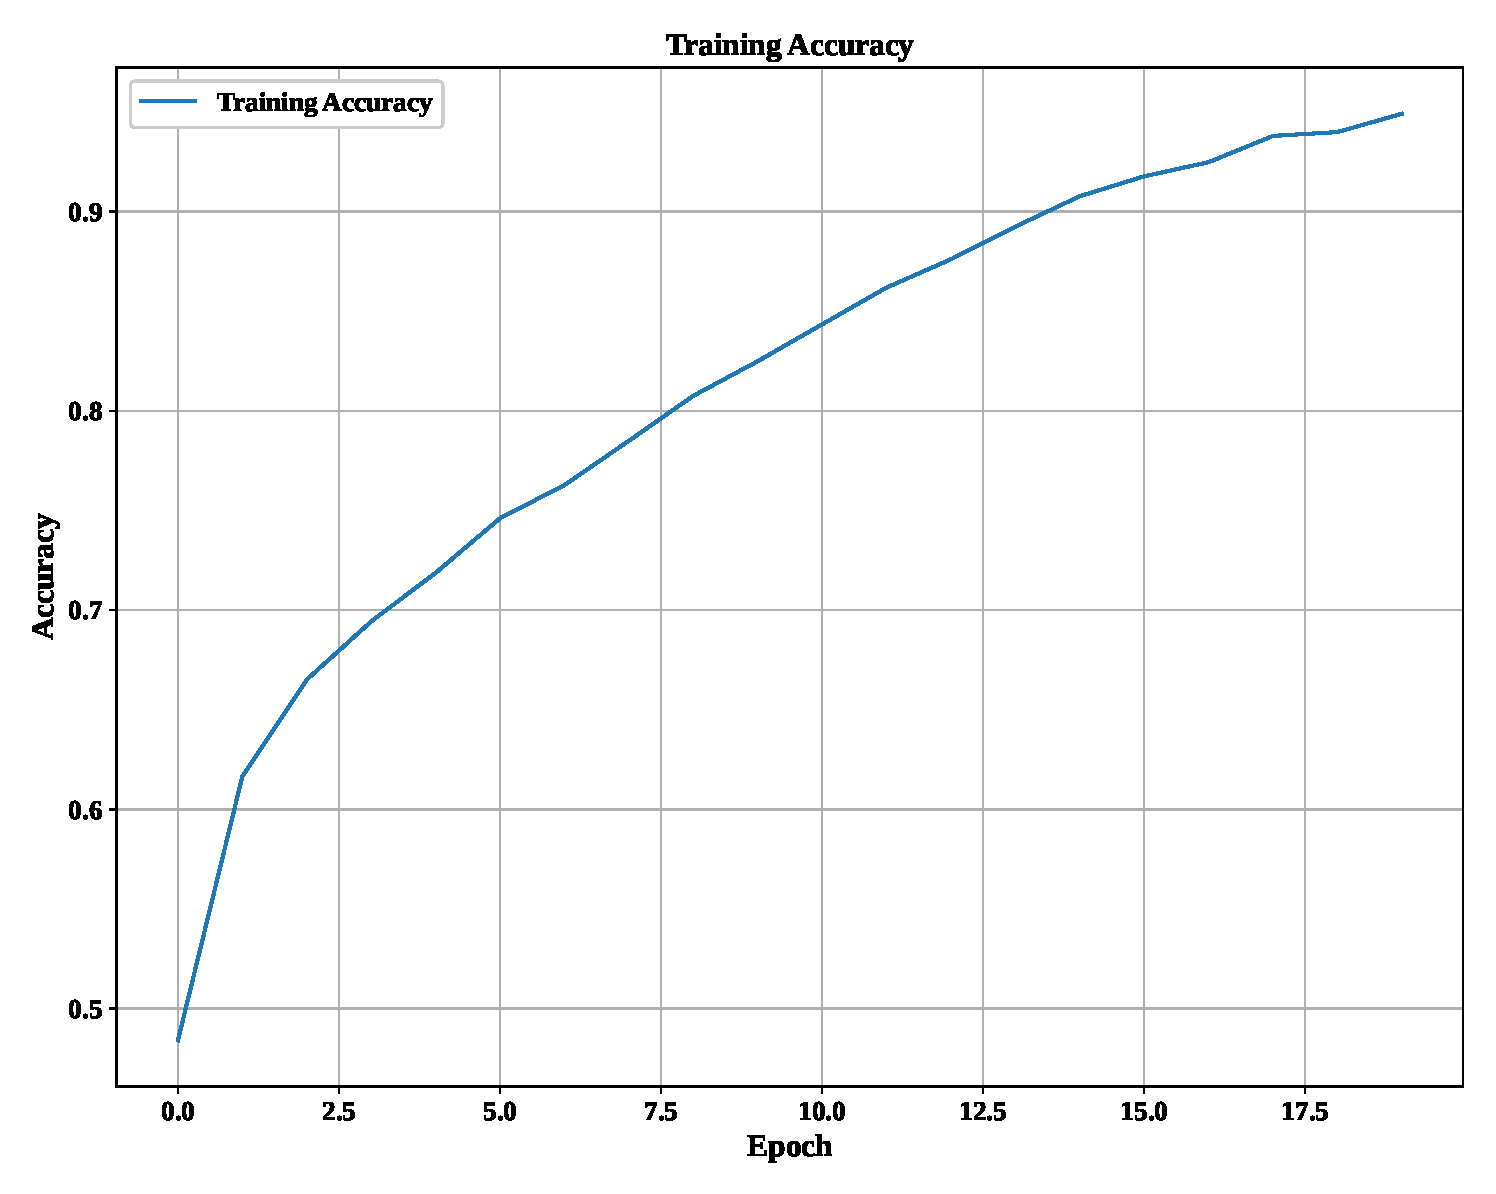
\includegraphics[width=\textwidth]{Training_Accuracy.eps}
\caption{Training Accuracy}
\end{figure}

\textbf{Interpretation:}

This plot shows the training accuracy progression over epochs, indicating how well the model learns from the training data. A rising trend suggests effective learning, while flattening or saturation may signal convergence or potential overfitting if validation accuracy doesn't follow similarly.

\subsection*{10.4 Validation Accuracy}

\begin{figure}[H]
\centering
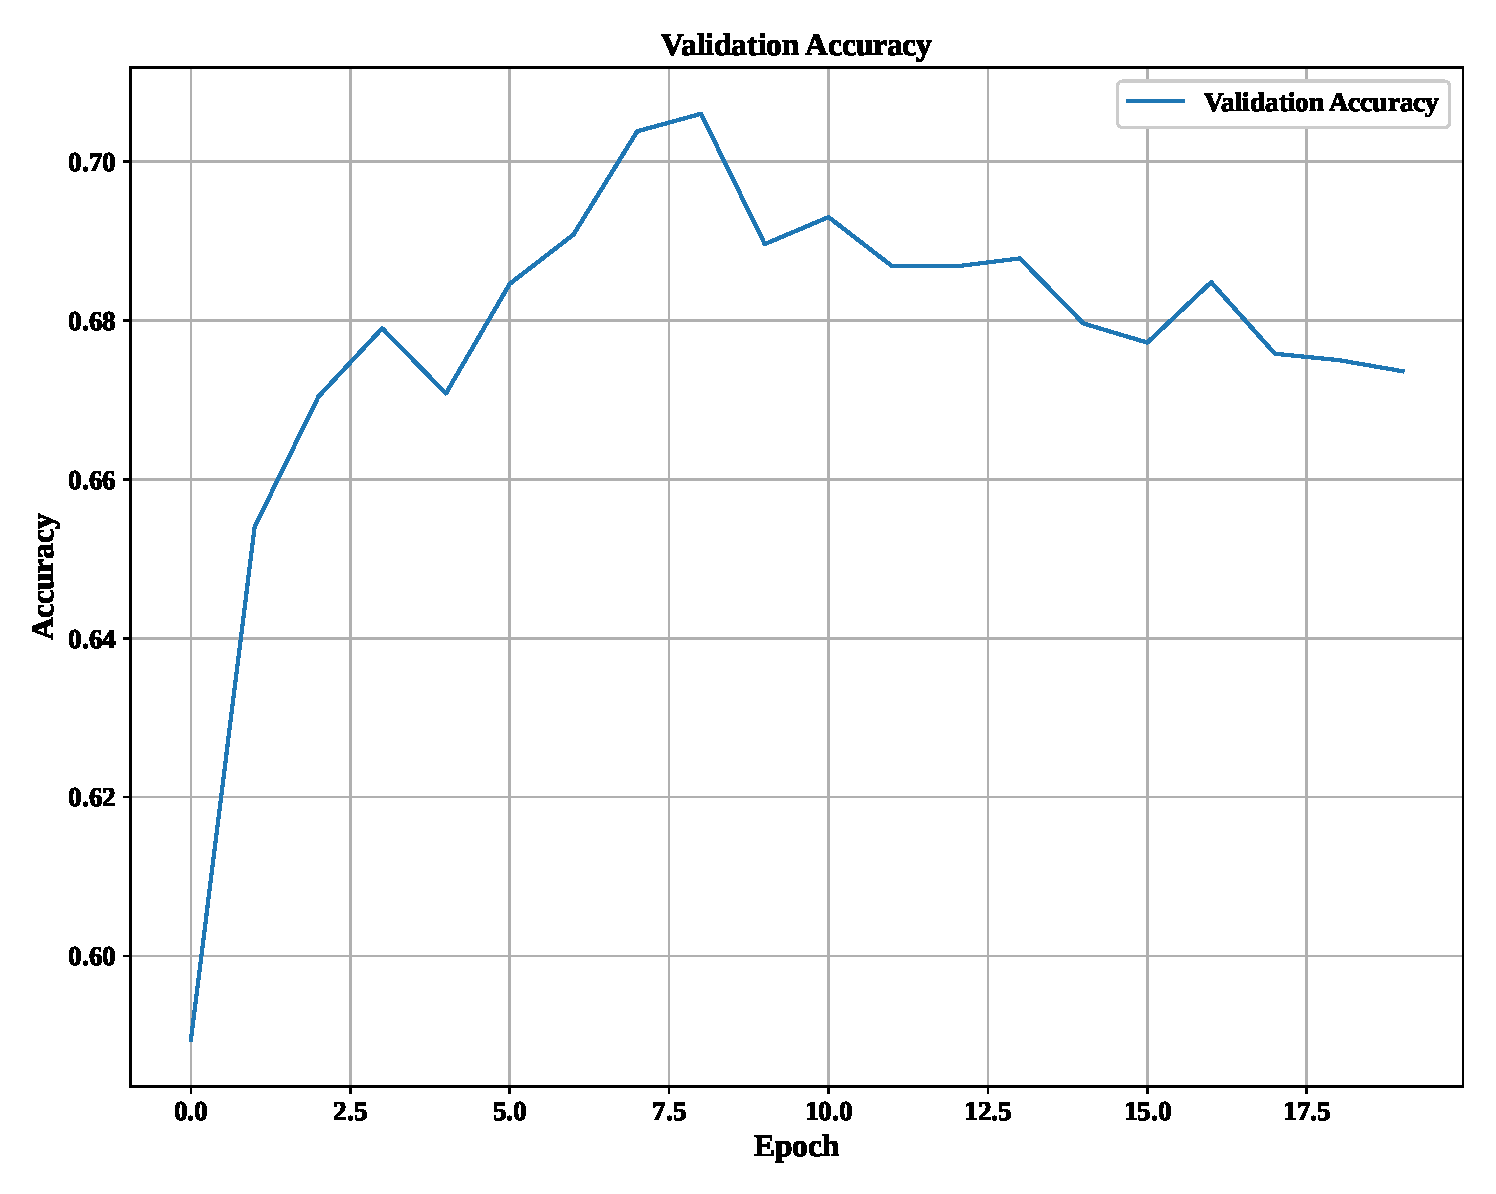
\includegraphics[width=\textwidth]{Validation_Accuracy.eps}
\caption{Validation Accuracy}
\end{figure}

\textbf{Interpretation:}

This graph shows how the validation accuracy changes over the course of the training. It reaches its point around the seventh epoch with a value of about 0.71. After that the accuracy slowly goes down. Stays between 0.68 and 0.69. The drop after the point means that the model might be overfitting.

\subsection*{10.5 Training Loss vs Epoch}

\begin{figure}[H]
\centering
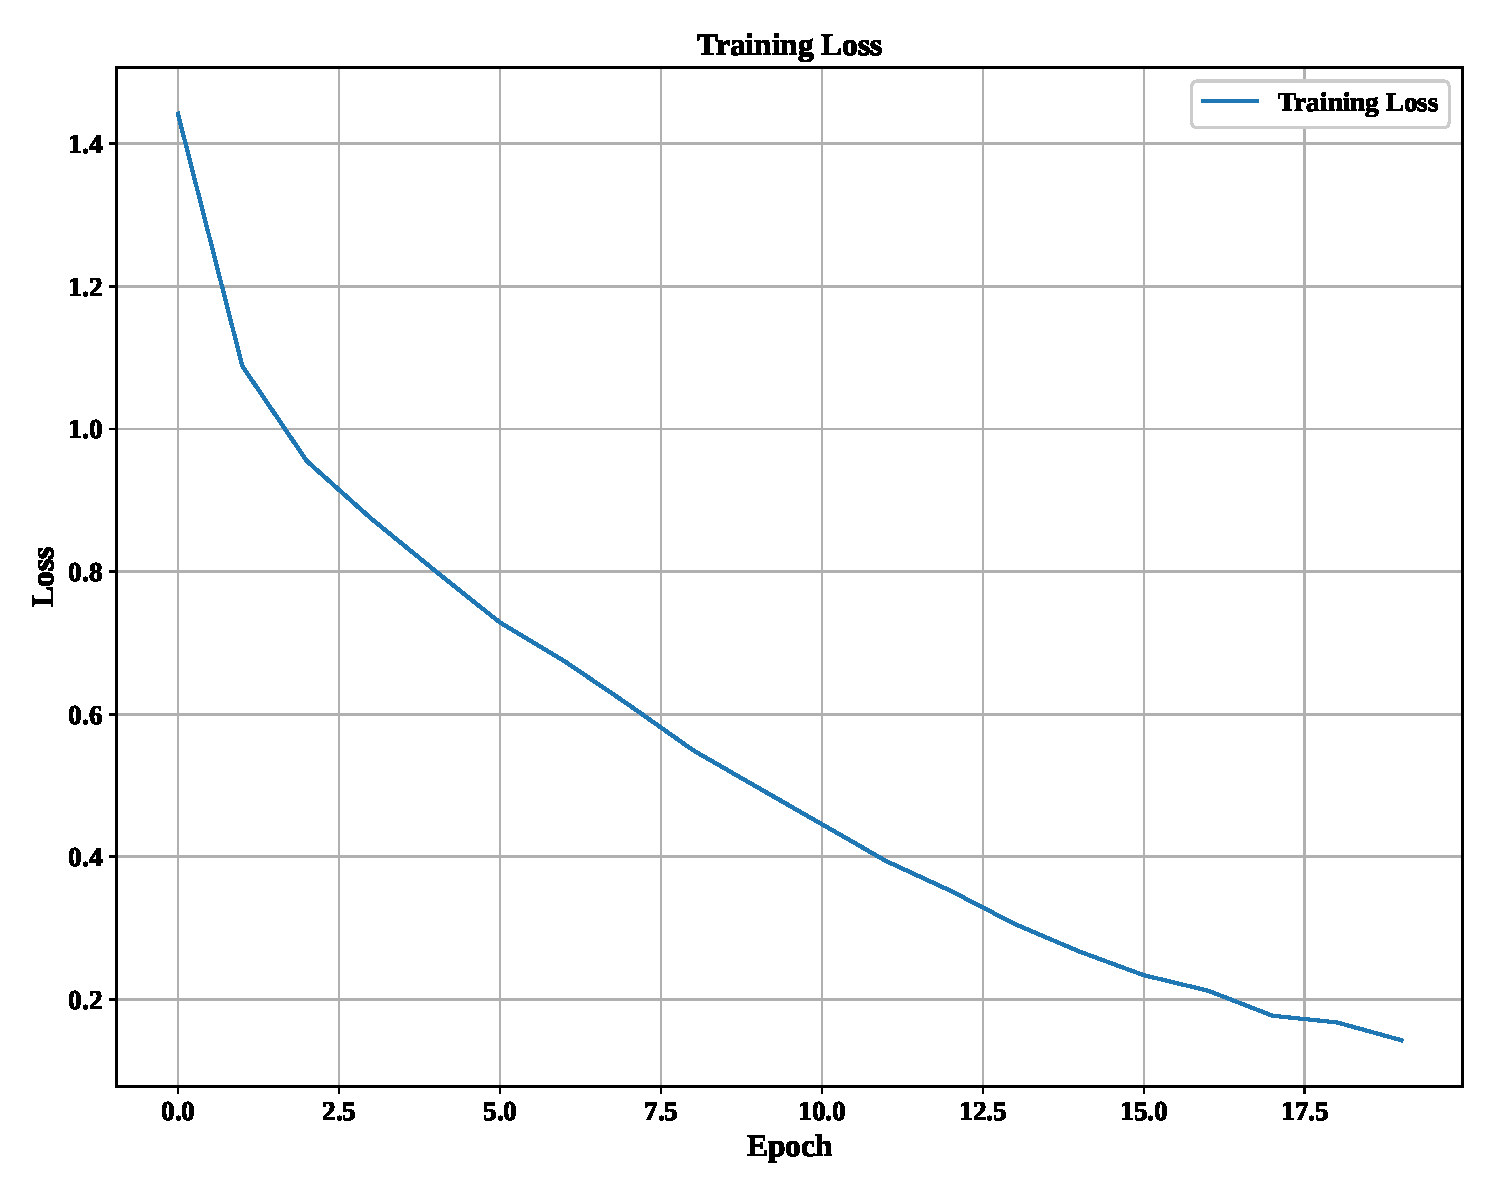
\includegraphics[width=\textwidth]{Training_Loss.eps}
\caption{Training Loss}
\end{figure}

\textbf{Interpretation:}

This plot shows a sharp decline in training loss during the initial epochs, followed by a gradual plateau as the model converges. The decreasing trend indicates effective learning, while the flattening near the end suggests the model has reached its optimal fit on the training data.

\subsection*{10.6 Validation Loss}

\begin{figure}[H]
\centering
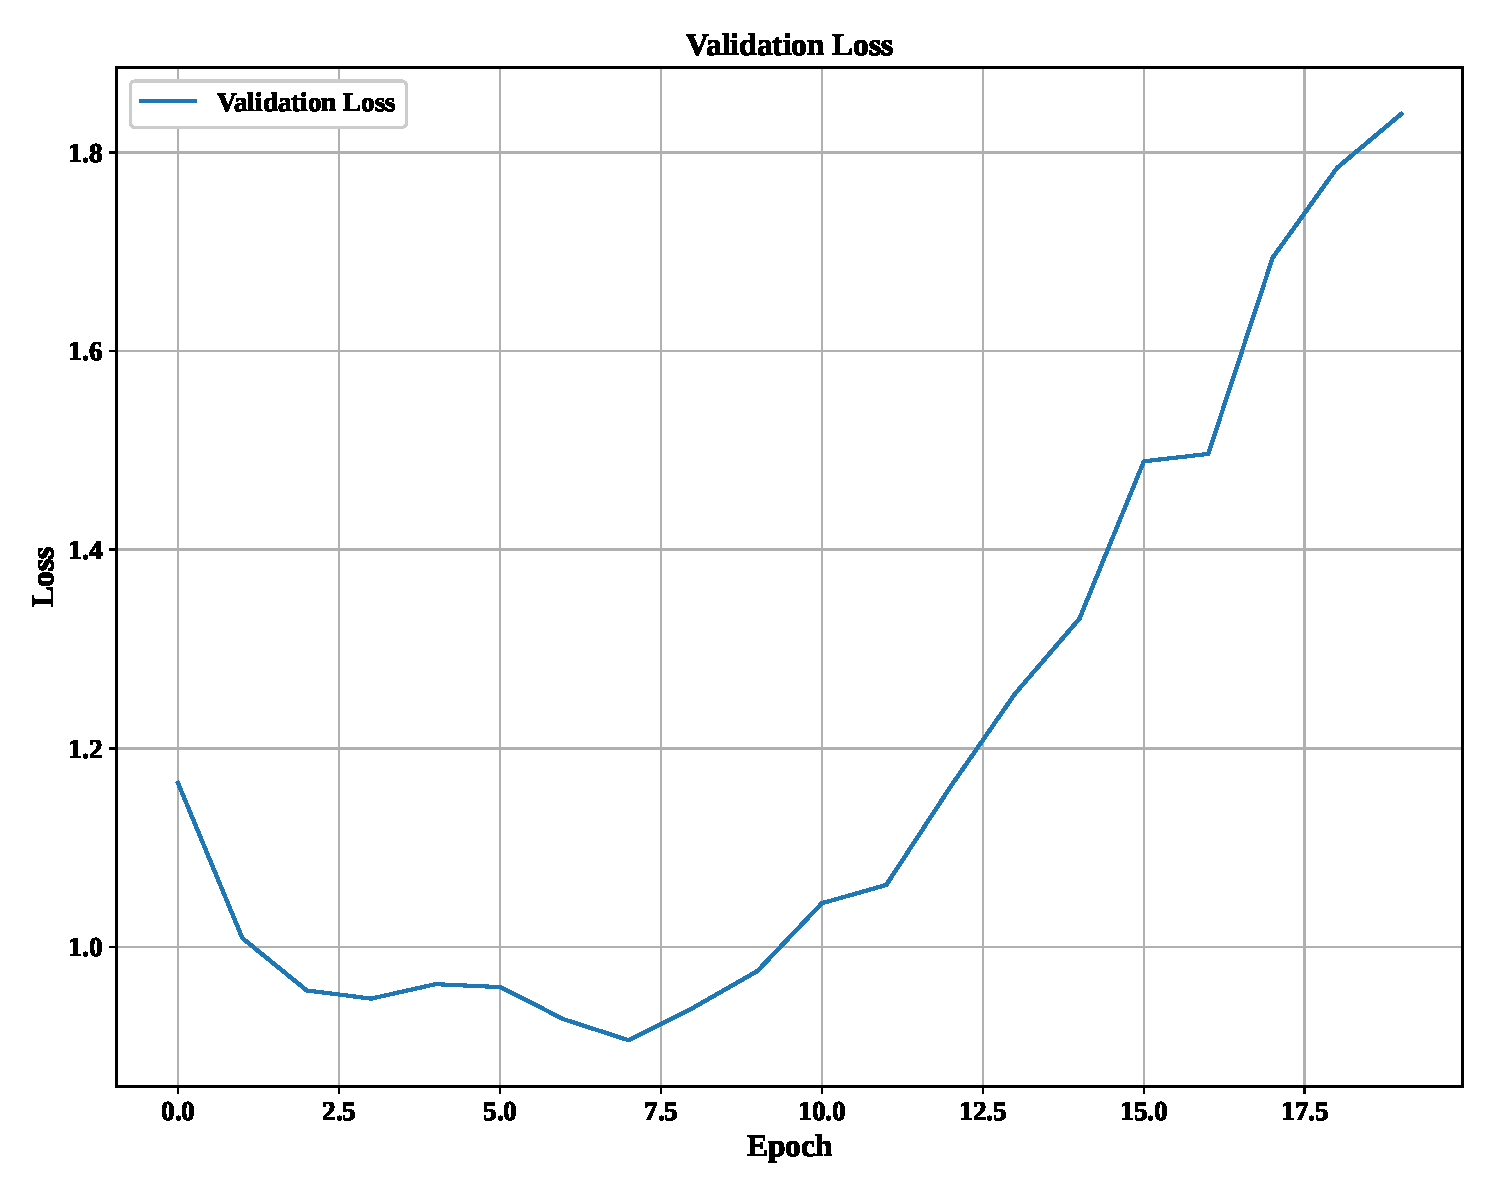
\includegraphics[width=\textwidth]{Validation_Loss.eps}
\caption{Validation Loss}
\end{figure}

\textbf{Interpretation:}

This plot shows validation loss decreasing to a minimum around epoch 7.5 (approximately 0.92), then steadily increasing to 1.80 by epoch 17.5. The clear upward trend after the minimum indicates significant overfitting, suggesting that model generalization deteriorates sharply with continued training beyond the optimal point.

\subsection*{10.7 Feature Map}

\begin{figure}[H]
\centering
\includegraphics[width=0.75\textwidth]{Feature_Maps.eps}
\caption{Feature Map}
\end{figure}

\textbf{Interpretation:}

This feature map displays 8 feature maps from a convolutional layer, each highlighting different learned patterns such as edges, textures, and shapes. The diversity across maps indicates that the model has learned a rich set of hierarchical features, with some maps capturing high-contrast boundaries while others focus on softer, more diffuse patterns.

\subsection*{10.8 Confusion Matrix}

\begin{figure}[H]
\centering

\includegraphics[width=0.75\textwidth]{Confusion_Matrix.eps}
\caption{Confusion Matrix}
\end{figure}

\textbf{Interpretation:}

This confusion matrix shows that the model performs best on classes like Airplane (714 correct), Automobile (781), and Ship (784), while struggling most with Cat (460) and Dog (516), which are frequently misclassified as each other. The high misclassification between visually similar categories (e.g., Cat$\leftrightarrow$Dog, Deer$\leftrightarrow$Horse) suggests the model has difficulty distinguishing fine-grained features among animal classes.

\section*{11. Additional Exercises}

\subsection*{Exercise 1: Output Size Calculation}

\textbf{Formula:}

\[
\text{Output Size}
=
\left\lfloor
\frac{N-K+2P}{S}
\right\rfloor+1
\]

where
$N=64$ (input size),
$K=5$ (kernel size),
$P=2$ (padding),
$S=2$ (stride).

\[
\begin{aligned}
\text{Output Size}
&=
\left\lfloor
\frac{64-5+2(2)}{2}
\right\rfloor+1\\
&=
\left\lfloor
\frac{64-5+4}{2}
\right\rfloor+1\\
&=
\left\lfloor
\frac{63}{2}
\right\rfloor+1\\
&=31+1\\
&=32
\end{aligned}
\]

\textbf{Answer:} The output feature map size is \textbf{$32\times32$}.

\subsection*{Exercise 2: Trainable Parameters Calculation}

\textbf{Formula:}

\[
\text{Parameters}
=
(K_h\times K_w\times C_{in}+1)\times C_{out}
\]

where
$K_h=K_w=3$,
$C_{in}=3$ (RGB channels),
$C_{out}=64$ (filters).

\[
\begin{aligned}
\text{Parameters}
&=
(3\times3\times3+1)\times64\\
&=
(27+1)\times64\\
&=
28\times64\\
&=
1792
\end{aligned}
\]

\textbf{Answer:} The convolution layer has \textbf{1792 trainable parameters}.

\subsection*{Exercise 3: ReLU vs Sigmoid Activation Functions}

\begin{table}[H]
\centering
\begin{tabular}{|p{3.5cm}|p{4.5cm}|p{4.5cm}|}
\hline
\textbf{Feature} & \textbf{ReLU} & \textbf{Sigmoid} \\
\hline
\textbf{Function} &
$f(x)=\max(0,x)$ &
$f(x)=\frac{1}{1+e^{-x}}$ \\
\hline
\textbf{Range} &
$[0,\infty)$ &
$(0,1)$ \\
\hline
\textbf{Computational Speed} &
Faster (simple threshold) &
Slower (exponential operation) \\
\hline
\textbf{Vanishing Gradient} &
Reduces vanishing-gradient problem for positive inputs &
Can suffer from vanishing gradients \\
\hline
\textbf{Sparsity} &
Promotes sparsity (neurons can die) &
Dense activations \\
\hline
\textbf{Common Use} &
Hidden layers in CNNs &
Output layer for binary classification \\
\hline
\textbf{Output Interpretation} &
Not probability-friendly &
Probability-friendly \\
\hline
\end{tabular}
\caption{Comparison of ReLU and Sigmoid Activation Functions}
\end{table}

\textbf{Interpretation:} ReLU is preferred for hidden layers due to faster computation and reduced vanishing gradient issues, while Sigmoid is typically used only at the output layer for binary classification tasks.

\subsection*{Exercise 4: Max Pooling vs Average Pooling}

\textbf{Results:}

\begin{itemize}
\item \textbf{Max Pooling Accuracy:} 0.6637 (66.37\%)
\item \textbf{Average Pooling Accuracy:} 0.6654 (66.54\%)
\end{itemize}

\textbf{Interpretation:} Average pooling performs slightly better than max pooling in this case (a marginal improvement of 0.17 percentage points).

\textbf{Analysis:}

\begin{itemize}
\item \textbf{Max Pooling} captures dominant features (edges, textures) but may lose subtle information.
\item \textbf{Average Pooling} retains more background context and spatial information.
\item Max pooling typically performs better for object recognition tasks, but the outcome can vary based on the dataset and model depth.
\end{itemize}

\subsection*{Exercise 5: Effect of Increasing Filters (16 $\rightarrow$ 64)}

\textbf{Results:}

\begin{itemize}
\item \textbf{Accuracy (16 filters):} Not explicitly provided (reference baseline)
\item \textbf{Accuracy (64 filters):} 0.6778 (67.78\%)
\item \textbf{Training Time:} 2864.64 seconds ($\sim$47.7 minutes)
\end{itemize}

\textbf{Interpretation:} Increasing convolution filters from 16 to 64 improves accuracy but at the cost of significantly higher computational expense.

\textbf{Analysis:}

\begin{itemize}
\item \textbf{Accuracy Improvement:} More filters allow the network to learn richer, more diverse feature representations, capturing finer patterns and complex hierarchies, which enhances model capacity and accuracy (67.78\%).
\item \textbf{Computation Cost:} Training time is substantially higher (2864 seconds) due to:
\begin{itemize}
\item 4$\times$ more filters in the layer
\item Increased memory bandwidth requirements
\end{itemize}
\end{itemize}

\section*{11. Results}

The final performance results of the CNN model are:

\begin{itemize}
\item \textbf{Training Accuracy:} 0.9492
\item \textbf{Testing Accuracy:} 0.6637
\item \textbf{Precision:} 0.6671
\item \textbf{Recall:} 0.6637
\item \textbf{F1-score:} 0.6639
\item \textbf{Number of Parameters:} 268650
\end{itemize}

\section*{12. Discussion}

\begin{enumerate}

\item \textbf{Why is convolution preferred over fully connected layers for images?}

Convolution is chosen since it maintains the spatial structure of images and is able to detect local features such as edges, textures, and shapes; it also makes use of shared weights, which greatly reduces the number of parameters when compared with fully connected layers.

\item \textbf{How does stride affect the feature map size?}

Strides refer to the distance by which the convolution filter slides over the input image. Strides that are larger will result in a smaller feature map, whereas smaller strides produce a larger feature map.

\item \textbf{What is the role of padding?}

Padding involves adding additional pixels, typically zeroes, around the edge of the input image. This ensures that spatial dimension is maintained, border features are taken into account, and prevents the shrinking of the feature map size.

\item \textbf{Why is pooling used?}

Pooling will reduce the spatial dimensions of feature maps, which will decrease computation and parameters involved. It will assist in maintaining the important features and offering translational invariance.

\item \textbf{How do feature maps represent image characteristics?}

Feature maps are representations of features captured by convolutional filters. The earlier layers usually capture simple features like edges and textures, whereas the deeper layers capture combinations of these features in order to capture complex features like shapes and objects.

\item \textbf{Why do CNNs require fewer parameters than MLPs?}

CNNs need fewer parameters due to the use of local connectivity and weight sharing in the convolutional layers. A single filter is applied on various parts of the image, while in MLP each neuron is connected to all the input pixels.

\end{enumerate}

\section*{13. References}

\begin{enumerate}
\item Goodfellow et al., \emph{Deep Learning}.
\item Bishop, \emph{Pattern Recognition and Machine Learning}.
\item Haykin, \emph{Neural Networks and Learning Machines}.
\item TensorFlow Documentation.
\item CIFAR-10 Dataset Documentation.
\end{enumerate}

\end{document}